\documentclass{article}
\usepackage[T1]{fontenc}
\usepackage{lmodern}
\usepackage{graphicx}
\usepackage{amsmath,amssymb}
\usepackage[a4paper,margin=2cm]{geometry}
\usepackage[absolute,overlay]{textpos}
\setlength{\TPHorizModule}{1mm}
\setlength{\TPVertModule}{1mm}
\usepackage[indonesian]{babel}
\usepackage{hyperref}
\setlength{\emergencystretch}{2em}
% unit: Halaman 20

\begin{document}

% === Halaman 20 (llm) ===

\vspace{261.36mm}

\section*{Program Caesar Cipher dalam Bahasa C++}

% deskripsi: Screenshot potongan kode program C++ untuk enkripsi Caesar Cipher yang mencakup fungsi enkripsi(), input pesan, jumlah pergeseran, dan loop untuk memproses setiap karakter alfabet.
% bbox normalisasi: [0.0400, 0.0900, 0.9200, 0.9700]
\begin{textblock*}{184.80mm}(8.40mm,26.73mm)
\noindent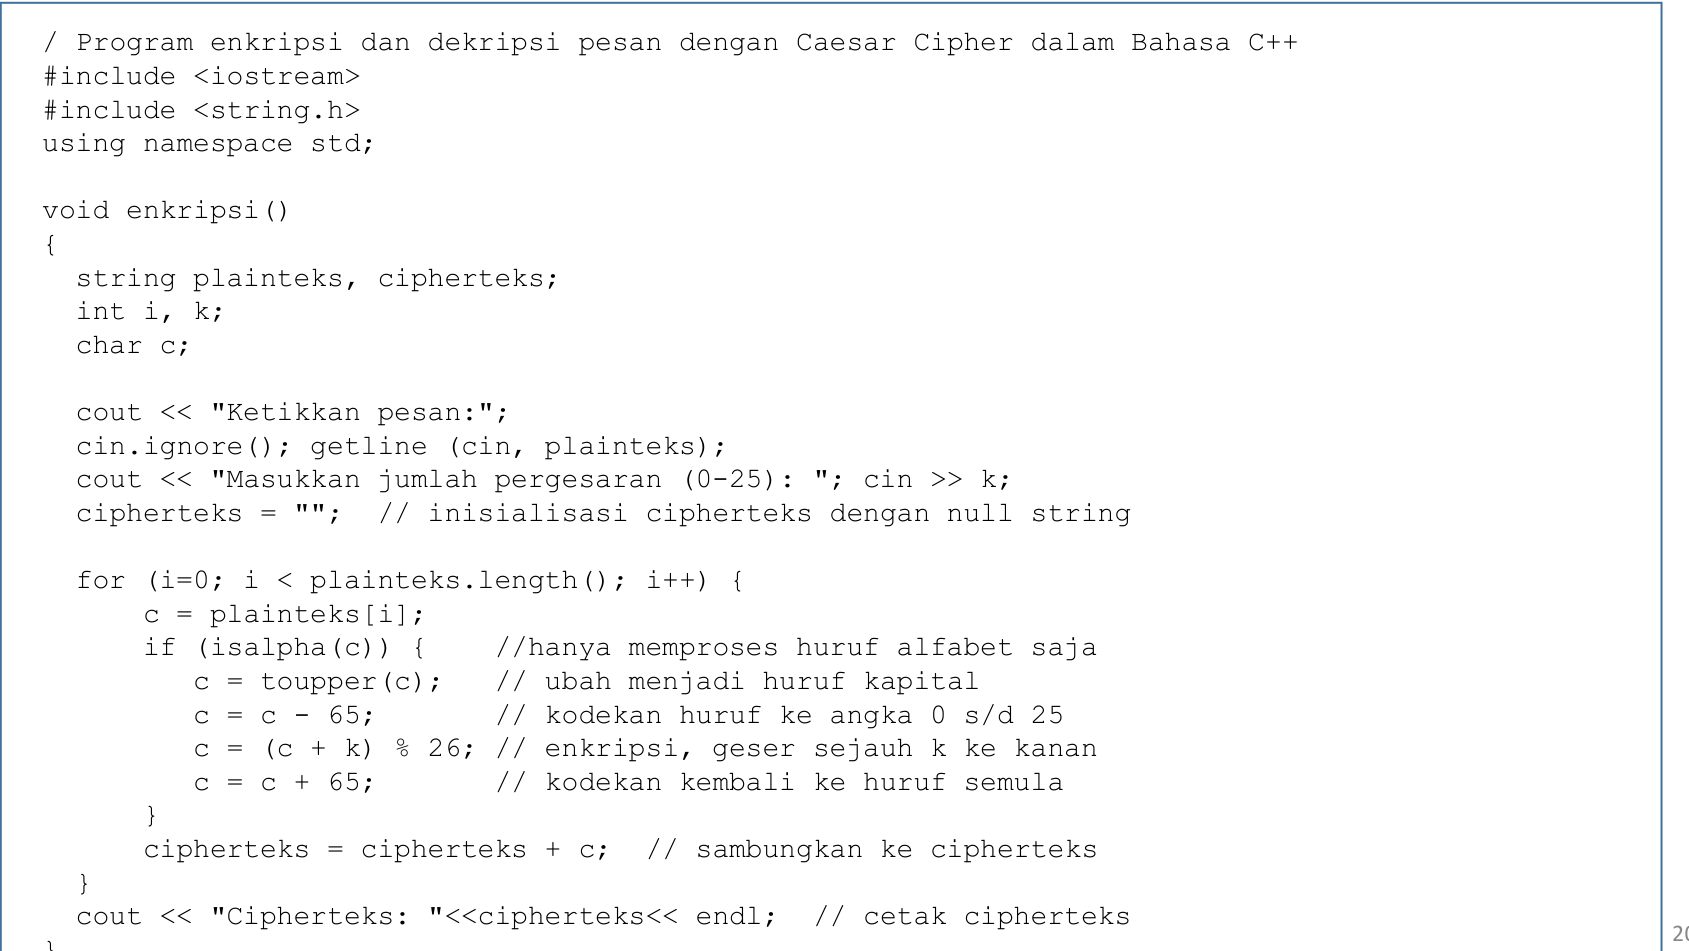
\includegraphics[width=184.80mm,height=261.36mm]{../../images/llm/page_020_img_01.png}%
\end{textblock*}

\end{document}
